\documentclass[pdf]{beamer}
%\documentclass[notes]{beamer}
%\documentclass{beamer}
\usepackage[utf8]{inputenc}
\usepackage{lmodern}
\usepackage{colortbl}
\usepackage{adjustbox}
%\usepackage{scrextend}
%\changefontsizes{7.5pt}


\makeatletter
\makeatother
\usepackage{graphicx}

\mode<presentation>{\usetheme{Warsaw}}
%\mode<presentation>{\usetheme{Madrid}}
%% preamble
\title{Métodos multivariados de Análisis de Datos}
\subtitle{Análisis de nutrientes en pizzas}

\author{
Ricardo Cruz Sánchez \\
  \and
Rolando Corona Jiménez
}

\institute[CIMAT]{CIMAT}

\AtBeginSection[]{%
\begin{frame}
    \tableofcontents[currentsection, subsectionstyle=show/show/hide]
\end{frame}
}

\begin{document}

\begin{frame}
\titlepage
\end{frame}

%\AtBeginSubsection[]
%{
%  \begin{frame}<beamer>
%    \frametitle{Contenido}
%    \tableofcontents[currentsection,currentsubsection]
%  \end{frame}
%}



\section{Introducción}
\begin{frame}{Bromatología}
Ciencia encargada del análisis de los nutrientes contenidos en los alimentos. Los estudios relacionados con esta disciplina cobran importancia al considerar que existen cantidades recomendadas en la ingesta diaria de cualquier individuo y el incremento o decremento de las cantidades repercute directamente en la salud del la persona
\end{frame}

\begin{frame}{}
\begin{itemize}

\item Particularmente, la pizza, tiende a ser uno de los alimentos con los cuales se sobrepasan los límites de nutrientes recomendados\\
\item En el presente trabajo, se considera una base de datos relativa a las pruebas nutrimentales realizadas en distintas pizzas y con base a estos datos se pretende realizar un análisis multivariado.
\end{itemize}

\end{frame}


\begin{frame}{Repositorio}
\begin{itemize}

\item https://github.com/rolandocj/proyecto-pizzas/tree/develop
\end{itemize}

\end{frame}



\section{Análisis exploratorio.}

\begin{frame}
\begin{itemize}
\item \textbf{Ident:} Variable tipo numérica, la cual corresponde a un identificador para cada pizza.
\item \textbf{HUMED:} Variable tipo numérica que indica el porcentaje de humedad contenido en la pizza.
\item \textbf{PROTE:} Variable tipo numérica que indica la cantidad de gramos de proteina contenida en 100g de pizza.
\item \textbf{GRASA:} Variable tipo numérica que indica la cantidad de gramos de grasa contenida en 100g de pizza.
\item \textbf{CENIZA:} Variable tipo numérica que indica la cantidad de gramos de ceniza contenida en 100g de pizza.
\item \textbf{SODIO:} Variable tipo numérica que indica la cantidad de gramos de sodio contenida en 100g de pizza.
\item \textbf{CARBO:} Variable tipo numérica que indica la cantidad de gramos de carbohidratos contenida en 100g de pizza.
\item \textbf{CALOR:} Variable tipo numérica que indica la cantidad de calorias contenida en 100g de pizza.
\item \textbf{MARCA:} Varibale tipo string, la cual indica la marca que fabrico la pizza. Es una variable categórica.
\end{itemize}
\end{frame}

\begin{frame}
\begin{figure}[h]
\centering
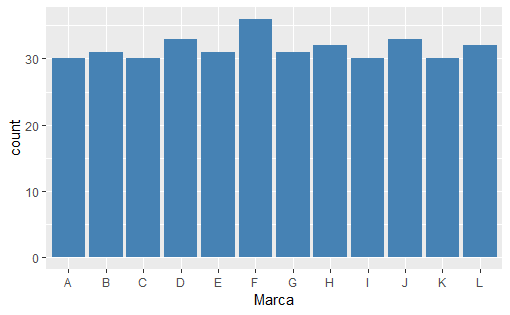
\includegraphics[scale=.65]{images/marca.png} 
\label{i1}
\caption{Conteo de registros por marca}
\end{figure}
\end{frame}

\begin{frame}
\begin{figure}[h]
\centering
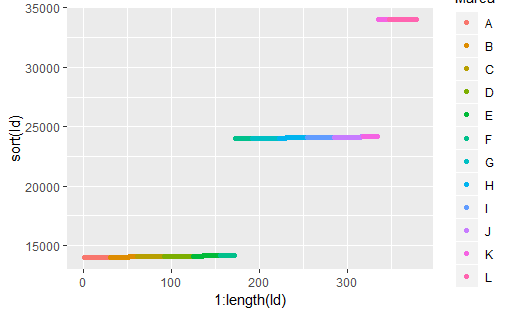
\includegraphics[scale=.65]{images/ident.png} 
\label{i2}
\caption{Comportamiento de la variable Ident de acuerdo a la marca}
\end{figure}
\end{frame}


\begin{frame}
\begin{figure}[h]
\centering
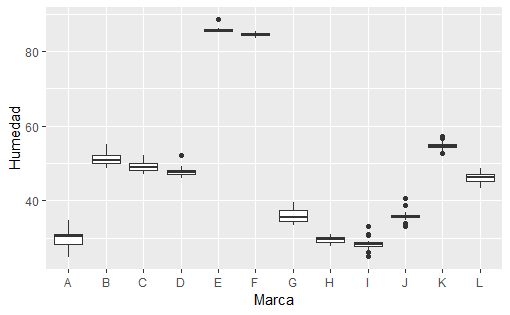
\includegraphics[scale=.65]{images/humed.png} 
\label{i3}
\caption{Comportamiento de la variable Humed de acuerdo a la marca}
\end{figure}
\end{frame}


\begin{frame}
\begin{figure}[h]
\centering
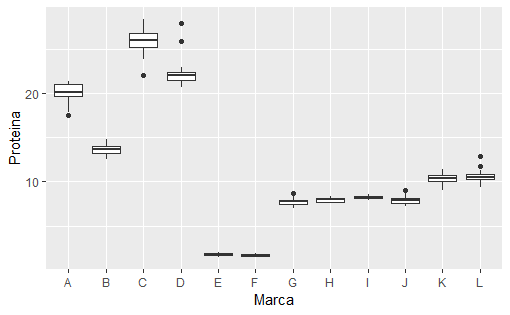
\includegraphics[scale=.65]{images/prote.png} 
\label{i4}
\caption{Comportamiento de la variable Prote de acuerdo a la marca}
\end{figure}
\end{frame}


\begin{frame}
\begin{figure}[h]
\centering
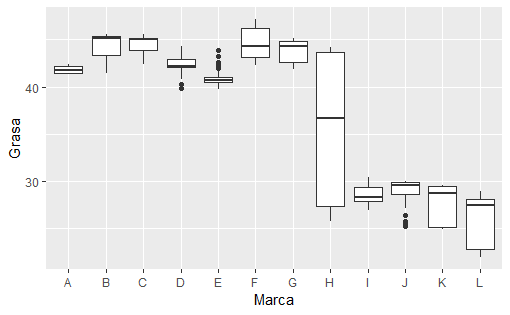
\includegraphics[scale=.65]{images/grasa.png} 
\label{i5}
\caption{Comportamiento de la variable Grasa de acuerdo a la marca}
\end{figure}
\end{frame}


\begin{frame}
\begin{figure}[h]
\centering
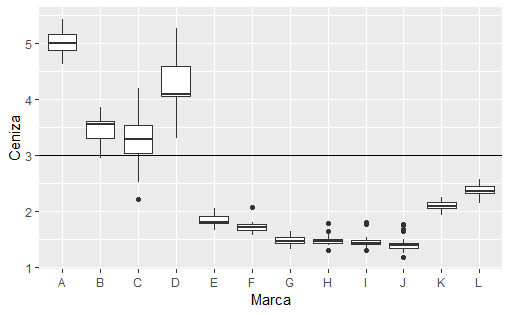
\includegraphics[scale=.65]{images/ceniz.png} 
\label{i6}
\caption{Comportamiento de la variable CENIZ de acuerdo a la marca}
\end{figure}
\end{frame}


\begin{frame}
\begin{figure}[h]
\centering
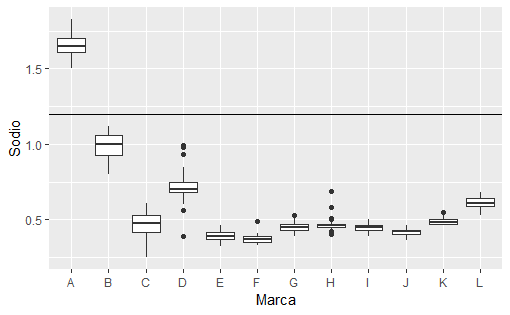
\includegraphics[scale=.65]{images/sodio.png} 
\label{i7}
\caption{Comportamiento de la variable sodio de acuerdo a la marca}
\end{figure}
\end{frame}

\begin{frame}
\begin{figure}[h]
\centering
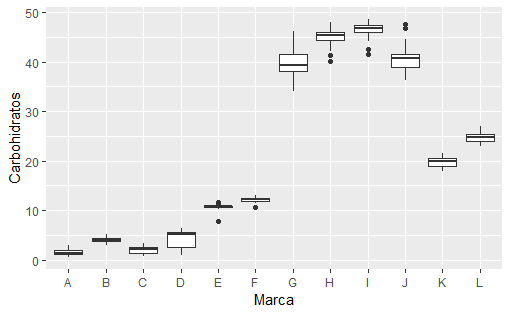
\includegraphics[scale=.65]{images/carbo.png} 
\label{i8}
\caption{Comportamiento de la variable Carbo de acuerdo a la marca}
\end{figure}
\end{frame}


\begin{frame}
\begin{figure}[h]
\centering
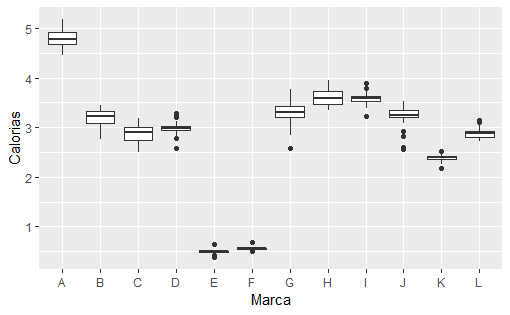
\includegraphics[scale=.65]{images/calor.png} 
\label{i9}
\caption{Comportamiento de la variable Calor de acuerdo a la marca}
\end{figure}
\end{frame}


\begin{frame}
\begin{figure}[h]
\centering
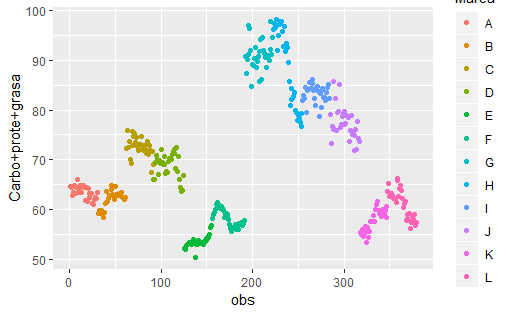
\includegraphics[scale=.65]{images/pgc.png} 
\label{i10}
\caption{Grasa+Proteina+Carbohidratos para cada observación}
\end{figure}
\end{frame}


\begin{frame}
\begin{table}[htbp]
\begin{center}
\begin{tabular}{|l|l|}
\hline
Nutriente&Error promedio\\ \hline\hline
Carbohidratos&1.37\\ \hline
Grasas&0.68\\ \hline
Proteina&0.04\\ \hline
\end{tabular}
\end{center}
\end{table}
\end{frame}

\begin{frame}
\begin{figure}[h]
\centering
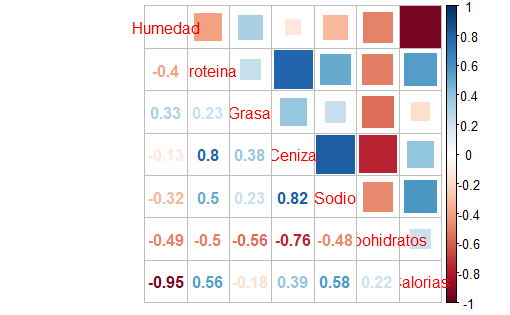
\includegraphics[scale=.65]{images/corr.png} 
\label{i11}
\caption{Correlación de las variables.}
\end{figure}
\end{frame}


\begin{frame}
\begin{itemize}
\item La relación entre humedad y calorías, tal vez corresponda a la presencia del fosfato, pues la presencia de fosfato modifica el valor de estas dos variables y se encuentra en alimentos como el queso y carnes.\\

\item La alta correlación entre Proteinas y cenizas puede ser explicado por la presencia de queso, pues es un alimento el cual es fuente de proteinas y minerales.\\

\item En el caso de la alta correlación entre sodio y cenizas, puede ser explicado por la presencia de tomate, ya que, este alimento eleva el valor de ambas variables.\\
\end{itemize}
\end{frame}

\section{Modelos de reducción de dimensiones.}

\subsection{Análisis de componentes principales (PCA)}

\begin{frame}{Cargas de componentes principales}
\begin{table}[ht]
\centering
\begin{tabular}{rrr}
  \hline
 & PC1 & PC2 \\ 
  \hline
Humedad & 0.21 & 0.58 \\ 
  Proteina & -0.47 & -0.03 \\ 
  Grasa & -0.19 & 0.41 \\ 
  Ceniza & -0.51 & 0.15 \\ 
  Sodio & -0.47 & -0.02 \\ 
  Carbohidratos & 0.32 & -0.49 \\ 
  Calorias & -0.34 & -0.48 \\ 
  Varianza acumulada & 48.64 \% &  83.59 \% \\ 
\end{tabular}
	\label{tabla:pesos_PCA}
	\caption{Pesos asociados a las primeras dos componentes principales.}
\end{table}
\end{frame}


\begin{frame}
\begin{figure}[h]
\centering
	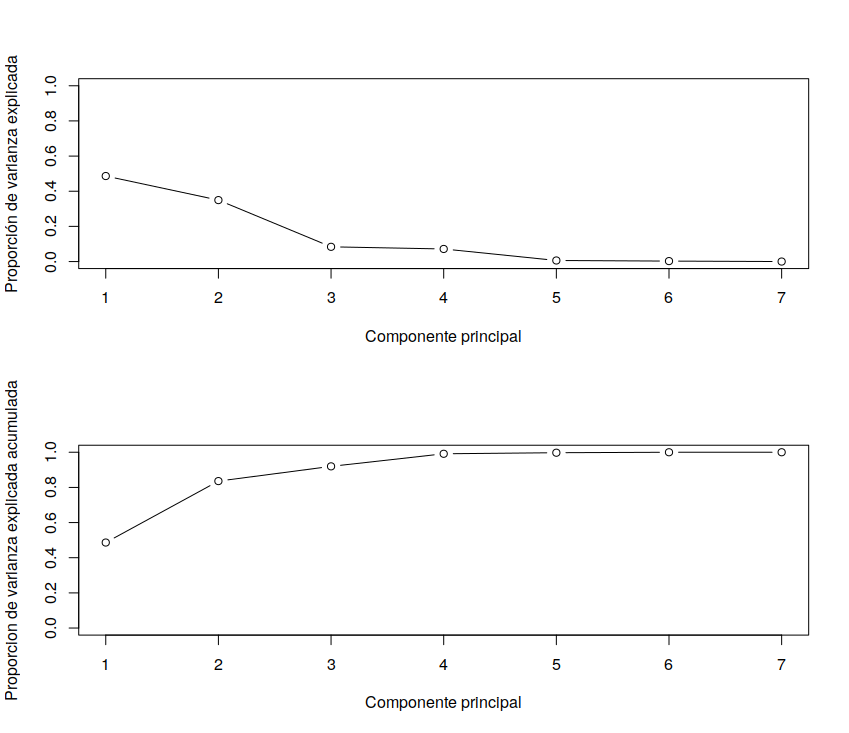
\includegraphics[scale=.35]{images/varPCA.png} 
	\label{i_var_PCA}
	\caption{Varianza explicada por las componentes principales}
\end{figure}
\end{frame}


\begin{frame}
\begin{figure}[h]
\centering
	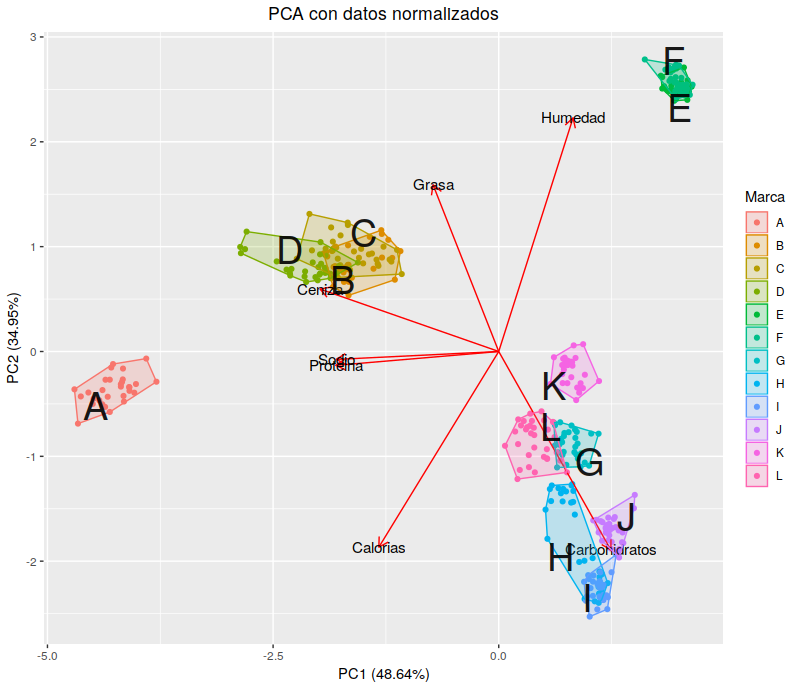
\includegraphics[scale=.35]{images/biplotPCA.png} 
	\label{i_biplot_PCA}
	\caption{Biplot PCA}
\end{figure}
\end{frame}

\subsection{Análisis Factorial}

\begin{frame}{Resumen de Análisis Factorial}
\begin{table}[ht]
\begin{adjustbox}{width= 4in,center}
\centering
\begin{tabular}{rrrrr}
  \hline
 & Factor1 & Factor2 & Varianza específica & Comunalidades \\ 
  \hline
Humedad & 0.06 & -1.00 & 0.01 & 1.00 \\ 
  Proteina & 0.76 & 0.44 & 0.23 & 0.77 \\ 
  Grasa & 0.47 & -0.30 & 0.69 & 0.31 \\ 
  Ceniza & 0.94 & 0.19 & 0.08 & 0.92 \\ 
  Sodio & 0.73 & 0.39 & 0.32 & 0.68 \\ 
  Carbohidratos & -0.90 & 0.44 & 0.01 & 1.00 \\ 
  Calorias & 0.23 & 0.97 & 0.01 & 0.99 \\     
  Prop. de Varianza  & 44 \% &  36.9 \% \\
  Var. acumulada & 44 \% &  80.9 \% \\ 
   \hline
\end{tabular}
\end{adjustbox}
	\label{tabla:factores}
	\caption{Resultados del análisis factorial.}	
\end{table}
\end{frame}

\begin{frame}{Aproximación a R}
\begin{table}[ht]
\begin{adjustbox}{width= 4in,center}
\centering
\begin{tabular}{rrrrrrrr}
  \hline
 & Humedad & Proteina & Grasa & Ceniza & Sodio & Carbohidratos & Calorias \\ 
  \hline
Humedad & -0.00 & -0.02 & 0.00 & -0.00 & 0.01 & -0.00 & -0.00 \\ 
  Proteina & -0.02 & 0.00 & -0.01 & -0.01 & -0.22 & -0.01 & -0.04 \\ 
  Grasa & 0.00 & -0.01 & 0.00 & -0.01 & -0.00 & -0.00 & 0.00 \\ 
  Ceniza & -0.00 & -0.01 & -0.01 & -0.00 & 0.06 & 0.00 & -0.00 \\ 
  Sodio & 0.01 & -0.22 & -0.00 & 0.06 & -0.00 & 0.01 & 0.04 \\ 
  Carbohidratos & -0.00 & -0.01 & -0.00 & 0.00 & 0.01 & -0.00 & -0.00 \\ 
  Calorias & -0.00 & -0.04 & 0.00 & -0.00 & 0.04 & -0.00 & 0.00 \\ 
   \hline
\end{tabular}
\end{adjustbox}
	\label{tabla:aproximacion}
	\caption{Diferencia entre R y $LL' + \Psi$, con redondeo a tres dígitos.}
\end{table}
\end{frame}

\begin{frame}
\begin{figure}[h]
\centering
	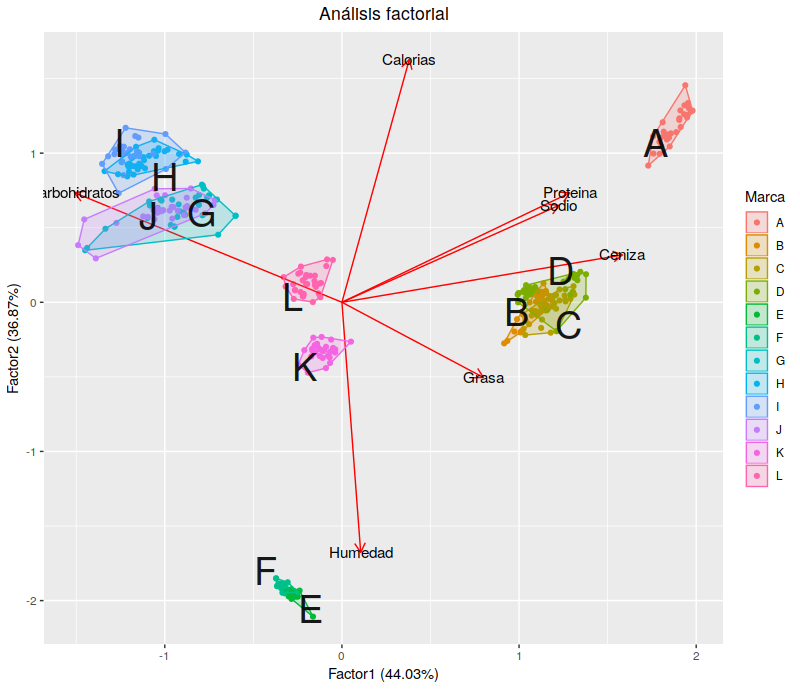
\includegraphics[scale=.35]{images/biplotFactores.png} 
	\label{i_biplot_Factores}
	\caption{Biplot usando 2 factores}
\end{figure}
\end{frame}

\section{Análisis por agrupación.}

\subsection{Elección del número de clusters}

\begin{frame}
\begin{figure}[h]
\centering
	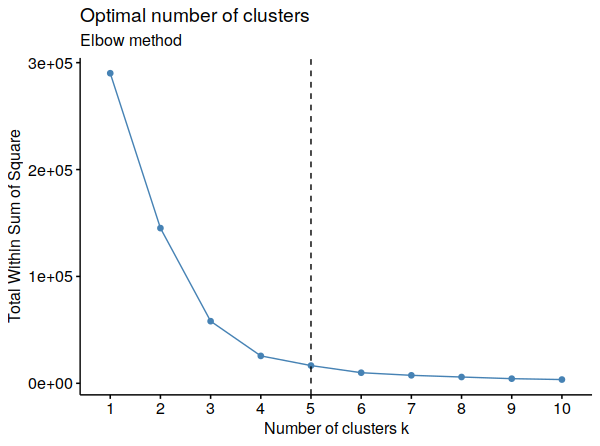
\includegraphics[scale=.5]{images/clusterElbow.png} 
	\label{i_cluster_Elbow}
	\caption{Suma total de cuadrados entre clústers vs número de clusters}
\end{figure}
\end{frame}

\begin{frame}
\begin{figure}[h]
\centering
	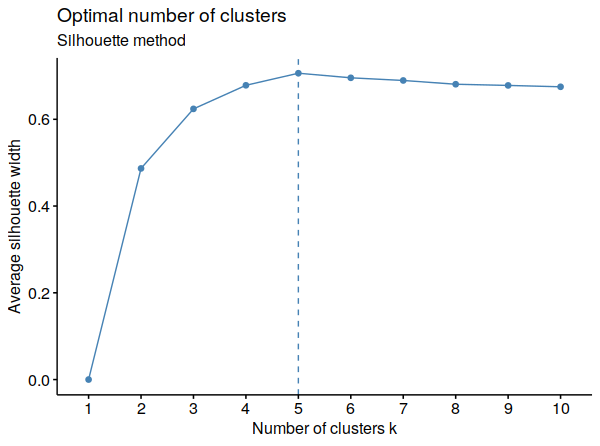
\includegraphics[scale=.5]{images/clusterSilhouette.png} 
	\label{i_cluster_Silhouette}
	\caption{Silhouette promedio vs número de clusters}
\end{figure}
\end{frame}


\subsection{Asignación de clusters}

\begin{frame}
\begin{figure}[h]
\centering
	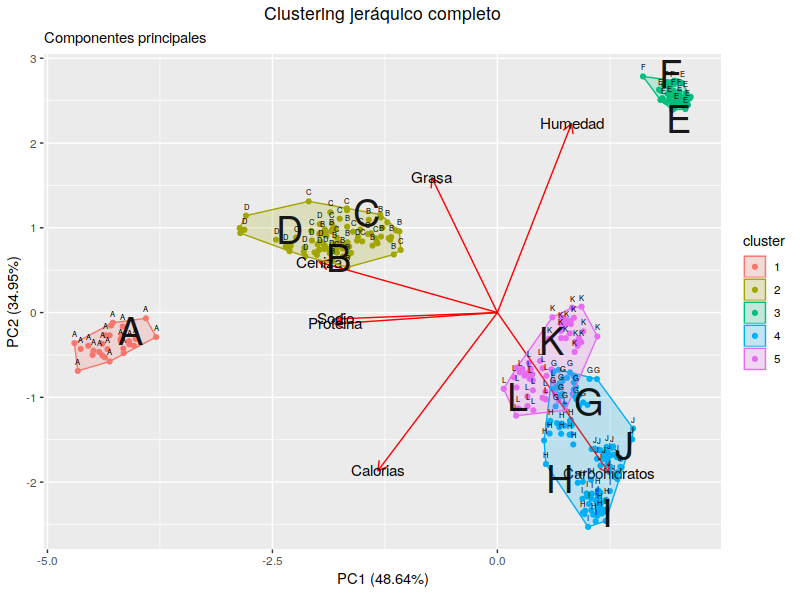
\includegraphics[scale=.35]{images/clusterPCA.png} 
	\label{i_cluster_PCA}
	\caption{Clustering jerárquico completo (Representación: PCA)}
\end{figure}
\end{frame}

\begin{frame}
\begin{figure}[h]
\centering
	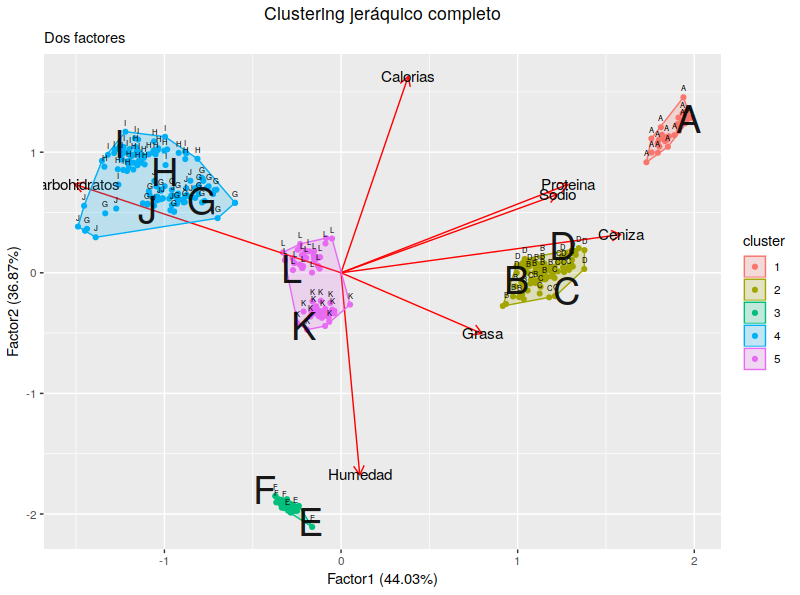
\includegraphics[scale=.35]{images/clusterFactores.png} 
	\label{i_cluster_Factores}
	\caption{Clustering jerárquico completo (Representación: Factores)}
\end{figure}
\end{frame}


\section{Modelos de clasificación.}
\subsection{LDA}
\begin{frame}

\begin{table}[ht]
\begin{adjustbox}{width= 3.5in,center}
\centering
\begin{tabular}{rrrrrrrrrrrrr}
  \hline
 & A & B & C & D & E & F & G & H & I & J & K & L \\ 
  \hline
A &   9 &   0 &   0 &   0 &   0 &   0 &   0 &   0 &   0 &   0 &   0 &   0 \\ 
  B &   0 &  17 &   0 &   0 &   0 &   0 &   0 &   0 &   0 &   0 &   0 &   0 \\ 
  C &   0 &   0 &  15 &   0 &   0 &   0 &   0 &   0 &   0 &   0 &   0 &   0 \\ 
  D &   0 &   0 &   1 &  19 &   0 &   0 &   0 &   0 &   0 &   0 &   0 &   0 \\ 
  E &   0 &   0 &   0 &   0 &  14 &   2 &   0 &   0 &   0 &   0 &   0 &   0 \\ 
  F &   0 &   0 &   0 &   0 &   1 &  16 &   0 &   0 &   0 &   0 &   0 &   0 \\ 
  G &   0 &   0 &   0 &   0 &   0 &   0 &  12 &   0 &   0 &   0 &   0 &   0 \\ 
  H &   0 &   0 &   0 &   0 &   0 &   0 &   0 &   8 &   9 &   0 &   0 &   0 \\ 
  I &   0 &   0 &   0 &   0 &   0 &   0 &   0 &   2 &  14 &   1 &   0 &   0 \\ 
  J &   0 &   0 &   0 &   0 &   0 &   0 &   0 &   0 &   0 &  13 &   0 &   0 \\ 
  K &   0 &   0 &   0 &   0 &   0 &   0 &   0 &   0 &   0 &   0 &  18 &   0 \\ 
  L &   0 &   0 &   0 &   0 &   0 &   0 &   0 &   0 &   0 &   0 &   0 &  18 \\ 
   \hline
\end{tabular}
\end{adjustbox}
	\label{tabla:confusionLDAtrain}
	\caption{Matriz de confusión LDA train}
\end{table}

error de clasificación:  0.08465608
\end{frame}

\begin{frame}
 \begin{table}[ht]
 \begin{adjustbox}{width= 3.5in,center}
\centering
\begin{tabular}{rrrrrrrrrrrrr}
  \hline
 & A & B & C & D & E & F & G & H & I & J & K & L \\ 
  \hline
A &  21 &   0 &   0 &   0 &   0 &   0 &   0 &   0 &   0 &   0 &   0 &   0 \\ 
  B &   0 &  14 &   0 &   0 &   0 &   0 &   0 &   0 &   0 &   0 &   0 &   0 \\ 
  C &   0 &   0 &  15 &   0 &   0 &   0 &   0 &   0 &   0 &   0 &   0 &   0 \\ 
  D &   0 &   0 &   1 &  12 &   0 &   0 &   0 &   0 &   0 &   0 &   0 &   0 \\ 
  E &   0 &   0 &   0 &   0 &  14 &   1 &   0 &   0 &   0 &   0 &   0 &   0 \\ 
  F &   0 &   0 &   0 &   0 &   0 &  19 &   0 &   0 &   0 &   0 &   0 &   0 \\ 
  G &   0 &   0 &   0 &   0 &   0 &   0 &  19 &   0 &   0 &   0 &   0 &   0 \\ 
  H &   0 &   0 &   0 &   0 &   0 &   0 &   0 &  11 &   4 &   0 &   0 &   0 \\ 
  I &   0 &   0 &   0 &   0 &   0 &   0 &   0 &   0 &  13 &   0 &   0 &   0 \\ 
  J &   0 &   0 &   0 &   0 &   0 &   0 &   0 &   0 &   0 &  20 &   0 &   0 \\ 
  K &   0 &   0 &   0 &   0 &   0 &   0 &   0 &   0 &   0 &   0 &  12 &   0 \\ 
  L &   0 &   0 &   0 &   0 &   0 &   0 &   0 &   0 &   0 &   0 &   0 &  14 \\ 
   \hline
\end{tabular}
\end{adjustbox}
	\label{tabla:confusionLDAtest}
	\caption{Matriz de confusión LDA test}
\end{table}
error de clasificación: 0.03157895
\end{frame}

\subsection{Multinomial}


\begin{frame}
\begin{table}[ht]
\begin{adjustbox}{width= 3.5in,center}
\centering
\begin{tabular}{rrrrrrrrrrrrr}
  \hline
 & A & B & C & D & E & F & G & H & I & J & K & L \\ 
  \hline
A &   9 &   0 &   0 &   0 &   0 &   0 &   0 &   0 &   0 &   0 &   0 &   0 \\ 
  B &   0 &  17 &   0 &   0 &   0 &   0 &   0 &   0 &   0 &   0 &   0 &   0 \\ 
  C &   0 &   0 &  15 &   0 &   0 &   0 &   0 &   0 &   0 &   0 &   0 &   0 \\ 
  D &   0 &   0 &   0 &  20 &   0 &   0 &   0 &   0 &   0 &   0 &   0 &   0 \\ 
  E &   0 &   0 &   0 &   0 &  16 &   0 &   0 &   0 &   0 &   0 &   0 &   0 \\ 
  F &   0 &   0 &   0 &   0 &   0 &  17 &   0 &   0 &   0 &   0 &   0 &   0 \\ 
  G &   0 &   0 &   0 &   0 &   0 &   0 &  12 &   0 &   0 &   0 &   0 &   0 \\ 
  H &   0 &   0 &   0 &   0 &   0 &   0 &   0 &  17 &   0 &   0 &   0 &   0 \\ 
  I &   0 &   0 &   0 &   0 &   0 &   0 &   0 &   0 &  17 &   0 &   0 &   0 \\ 
  J &   0 &   0 &   0 &   0 &   0 &   0 &   0 &   0 &   0 &  13 &   0 &   0 \\ 
  K &   0 &   0 &   0 &   0 &   0 &   0 &   0 &   0 &   0 &   0 &  18 &   0 \\ 
  L &   0 &   0 &   0 &   0 &   0 &   0 &   0 &   0 &   0 &   0 &   0 &  18 \\ 
   \hline
\end{tabular}
\end{adjustbox}
	\label{tabla:confusionMLtrain}
	\caption{Matriz de confusión Multinomial train}
\end{table}

error de clasificación: 0
\end{frame}

\begin{frame}
\begin{table}[ht]
\begin{adjustbox}{width= 3.5in,center}
\centering
\begin{tabular}{rrrrrrrrrrrrr}
  \hline
 & A & B & C & D & E & F & G & H & I & J & K & L \\ 
  \hline
A &  21 &   0 &   0 &   0 &   0 &   0 &   0 &   0 &   0 &   0 &   0 &   0 \\ 
  B &   0 &  14 &   0 &   0 &   0 &   0 &   0 &   0 &   0 &   0 &   0 &   0 \\ 
  C &   0 &   0 &  15 &   0 &   0 &   0 &   0 &   0 &   0 &   0 &   0 &   0 \\ 
  D &   0 &   0 &   1 &  12 &   0 &   0 &   0 &   0 &   0 &   0 &   0 &   0 \\ 
  E &   0 &   0 &   0 &   0 &  15 &   0 &   0 &   0 &   0 &   0 &   0 &   0 \\ 
  F &   0 &   0 &   0 &   0 &   1 &  18 &   0 &   0 &   0 &   0 &   0 &   0 \\ 
  G &   0 &   0 &   0 &   0 &   0 &   0 &  19 &   0 &   0 &   0 &   0 &   0 \\ 
  H &   0 &   0 &   0 &   0 &   0 &   0 &   0 &   9 &   6 &   0 &   0 &   0 \\ 
  I &   0 &   0 &   0 &   0 &   0 &   0 &   0 &   0 &  13 &   0 &   0 &   0 \\ 
  J &   0 &   4 &   0 &   0 &   0 &   2 &   0 &   0 &   0 &  14 &   0 &   0 \\ 
  K &   0 &   0 &   0 &   0 &   0 &   0 &   0 &   0 &   0 &   0 &  12 &   0 \\ 
  L &   0 &   0 &   0 &   0 &   0 &   0 &   0 &   0 &   0 &   0 &   0 &  14 \\ 
   \hline
\end{tabular}
\end{adjustbox}
	\label{tabla:confusionMLtest}
	\caption{Matriz de confusión Multinomial test}
\end{table}

error de clasificación: 0.07368421
\end{frame}

\subsection{Validación cruzada con caret}

\begin{frame}
\begin{table}[ht]
\centering
\begin{tabular}{rrrrrrrrrrrrr}
  \hline
Clasificador & Accuracy\\ 
  \hline
rn &   0.2953684  \\ 
mr &   0.9626203  \\ 
lda &   0.9498792 \\ 
rf &   0.9709806 \\ 
tree &   0.8468115\\ 
   \hline
\end{tabular}
	\label{tabla:AccuracyCV}
	\caption{Accuracy usando validación cruzada}
\end{table}
\end{frame}


\begin{frame}
\end{frame}

\section{Regresión Multivariada}
\subsection{MANOVA}
\begin{frame}
$$H_0:\mu_1=\hdots=\mu_12$$

\end{frame}

\begin{frame}
\begin{itemize}
\item ANOVA
\item MANOVA
\item MANOVA $2^{k-1}$
\end{itemize}
\end{frame}

\begin{frame}
$J$ y $G$.  Humedad, Proteina, Calorias y Carbohidratos por separado y aun nivel de significancia del .05.
\end{frame}

\subsection{Regresión}
\begin{frame}
Se consideraron como variables regresoras a aquellas que son nutrientes, a saber, Proteinas, Grasas, Sodio y Carbohidratos. Mientras que las variables dependientes serán Humedad, Cenizas y Calorias.
\end{frame}

\begin{frame}
\begin{itemize}
\item Para las 3 variables dependientes, se encontró que la variables Grasa no es significativa para el modelo
\item $R^2$ de $0.96$, $0.94$ y $0.93$
\end{itemize}
\end{frame}
\end{document}
